\Author{\daAuthorTwo}

In this section of our thesis, the functional implementation of the mobile app will be described. We will show how the FlutterMap component is built and what logic works in the background.

\subsection{Address-Provider}

Since without data, our app would be useless, we will start with describing the Address-Provider class. It is implemented using the \texttt{provider package} by Flutter. With its help, we can easily notify all screens and widgets when the data was updated.

\blankLine

The main objective of the Address-Provider is to communicate with the backend and GraphHopper instance, but also to bring the received data into the correct format for our frontend. For this, we defined four different instance variables. A list that stores all addresses, one that only holds the coordinates of the \texttt{border addresses} returned by the backend, a map that is used for coordinates of the routing points for a specific street (\textit{Map<String[street name]>, List<LatLng>[coordinates]}) and finally a map for storing the addresses grouped by their street. Every component that owns an instance of this Address Provider can access these variables, which makes it easy to display the data.

\blankLine

Due to the fact that the backend returns the addresses unsorted, the Address Provider also takes on this task. For the grouping by the street name, we can just use the map from before, but to then also sort the addresses ascending by their house number, we needed to write a function to compare them.

\blankLine

The \textit{compareHouseNumbers} function performs natural sorting of house numbers by splitting them into alternating numeric and non-numeric components. It achieves this using a regular expression that extracts sequences of digits and non-digit characters separately. The function then iterates through these parts, comparing numeric segments as integers to ensure correct numerical order and comparing non-numeric segments lexicographically. This approach ensures that house numbers such as "10a" and "10c" are sorted in an intuitive order, with "10a" preceding "10c". If all corresponding parts are equal, the function resolves ties by comparing the lengths of the extracted parts lists. This method improves the readability and usability of address lists by maintaining a logical, human-friendly order.

\lstset{style=generic, caption=compareHouseNumbers function (AddressProvider.dart)}
\begin{lstlisting}
    int compareHouseNumbers(String a, String b) {
        final regex = RegExp(r'(\d+|\D+)');
    
        final partsA = regex.allMatches(a).map((match) => match.group(0)!).toList();
        final partsB = regex.allMatches(b).map((match) => match.group(0)!).toList();
    
        for (int i = 0; i < partsA.length && i < partsB.length; i++) {
          final partA = partsA[i];
          final partB = partsB[i];
    
          //compare numeric part
          if (int.tryParse(partA) != null && int.tryParse(partB) != null) {
            final numA = int.parse(partA);
            final numB = int.parse(partB);
            if (numA != numB) return numA.compareTo(numB);
          } else {
            // Compare alphabetic part
            final comparison = partA.compareTo(partB);
            if (comparison != 0) return comparison;
          }
        }
    
        return partsA.length.compareTo(partsB.length);
      }
\end{lstlisting}

\subsection{HTTP-Requests}

To actually access the data from our database, we built our backend API. It can be accessed through different HTTP-Requests. The mobile application makes use of the following routes: 

\begin{itemize}
    \item \textbf{fetch all addresses of area}
    
    As the name suggests, it fetches and saves all addresses from the area that is set through the QR-Code. Here the \textit{compareHouseNumbers} function gets used.

    \lstset{style=generic, caption=use of compareHouseNumbers function (AddressProvider.dart)}
    \begin{lstlisting}
        addressMap = groupBy(addresses, (Address address) => address.street.name);

        addressMap = addressMap.map((key, value) {
          value.sort((a, b) => compareHouseNumbers(a.houseNumber, b.houseNumber));
          return MapEntry(key, value);
        });
    \end{lstlisting}

    \item \textbf{fetch border addresses of area}
    Fetches and extracts the coordinates of the border addresses returned by the backend.

    \lstset{style=generic, caption=extraction of coordinates from border addresses (AddressProvider.dart)}
    \begin{lstlisting}
        borderAddresses = decodedJSON.map((json) => Address.fromJson(json)).toList().map((point) => LatLng(point.latitude, point.longitude)).toList();
    \end{lstlisting}

    \item \textbf{toggle address visited state}
    
    Used by the list screen, on swipe of an individual address-item.

    \item \textbf{toggle street visited state}
    Virtually the same as the toggle address, but now for the whole street. Gets called when a user swipes and confirms the change on a whole street.

    \item \textbf{update comment of address}
    
    Used by the \textit{details pop-up} on save with a new comment in the text field.

    \item \textbf{fetch route information for streets}
    
    Call to our GraphHopper instance. Iterates over every key of the \textit{addressMap}, requests the routing data, and calls the function \textit{extractPoints} to extract only valid data out of the whole JSON response.
\end{itemize}

\subsubsection{Performance}
To improve our performance, the first thing to change would be to move away from HTTP-Request to Web-Sockets. This would be a more suitable technology since only when the data on the server updates do we get an HTTP-Frame. Through this change, we could drastically minimize the traffic our app produces, as well as the performance, since the widgets do not need to re-render constantly.   

\subsection{Implementation of the FlutterMap Component}

The FlutterMap widget is built up in layers, which all can be individually ordered and configured. In this part, the layers that we utilized and the configuration options we set will be described. 

\begin{itemize}
  \item \textbf{Tile-Layer}
  
  This layer imports the tiles, so the actual map of OpenStreetMap's tile server. In future iterations, a different server or tile style (vector tiles) could be used to improve performance and usability further.

  \item \textbf{Polygon-Layer}
  
  In this layer, we draw the polygon that marks the border of the selected area. To achieve this, we just create a new Polygon object with the coordinates saved in the \textit{borderAddresses} list of the \textit{AddressProvider} and set a few styling options, like the stroke width and border color.

  \item \textbf{Polyline-Layer}
  
  This layer was utilized to display the streets that correspond to the specified area. Here we draw different polylines based on the routing data we fetched from our GraphHopper server. In the future, this feature could be further improved so different streets get drawn in varying colors. For now, every street polyline gets displayed in blue. 

  \item \textbf{Marker-Layer}
  
  This is the final and arguably most important layer because here we set a marker for every address. This marker can vary, depending on the specification that the admin assigned to an address in the Admin Panel. This was implemented by decoding the Base64 string, which is saved in the address object and stores the marker image. Additionally, if a comment is saved in the address, a little warning indicator gets displayed on the upper right-hand side of this encoded image. This got introduced so that users could see at a glance if there was something special to know about an address. We solved this by using a Stack widget. Additionally, we added a GestureDetector on top of this stack. This is used to open the details' dialog in which the user can modify the comment field. 
\end{itemize}

\subsection{Implementation of the List Screen}

Now, we will take a look through our list component. The interactive elements here are the two \textit{Dismissible} containers as well as the icon that indicates if an address has been visited.

The logic behind the color-coded \textit{Dismissibles} is just based on the \textit{alreadyVisited} attribute of the address. There is also a function (\textit{isWholeStreetVisited}) that checks if every address of a street has already been visited. When the users swipe the street item, a dialog gets displayed that prompts the user to confirm their action to avoid accidental swipes.

\begin{figure}[H]
  \centering
  \begin{minipage}{0.3\textwidth}
      \centering
      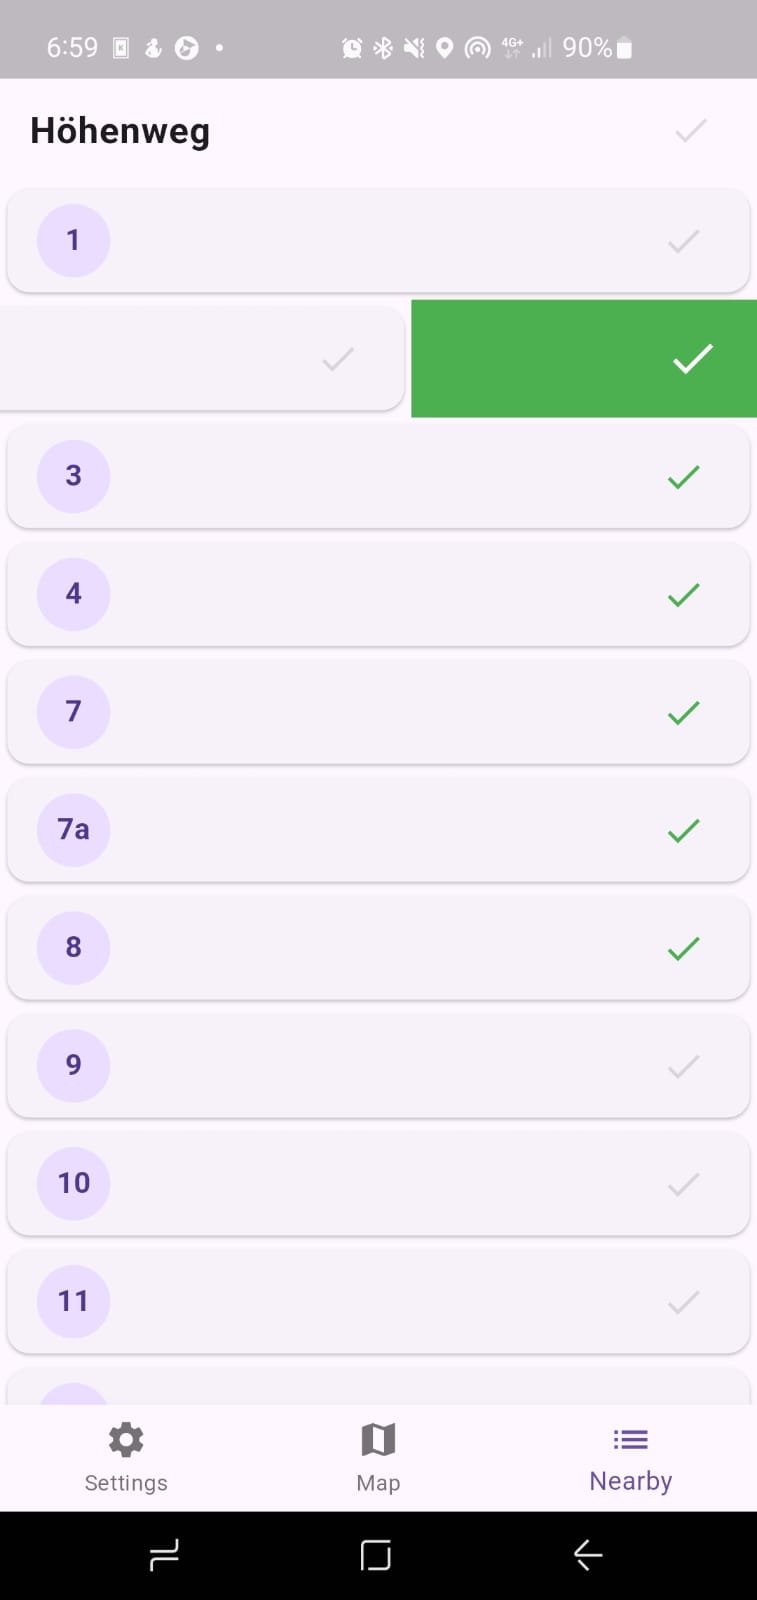
\includegraphics[width=\textwidth]{images/paul/listScreen/setIsVisitedTrue.jpeg}
      \caption{Setting \textit{alreadyVisited} true}
  \end{minipage}
  \hspace{2cm}
  \begin{minipage}{0.3\textwidth}
      \centering
      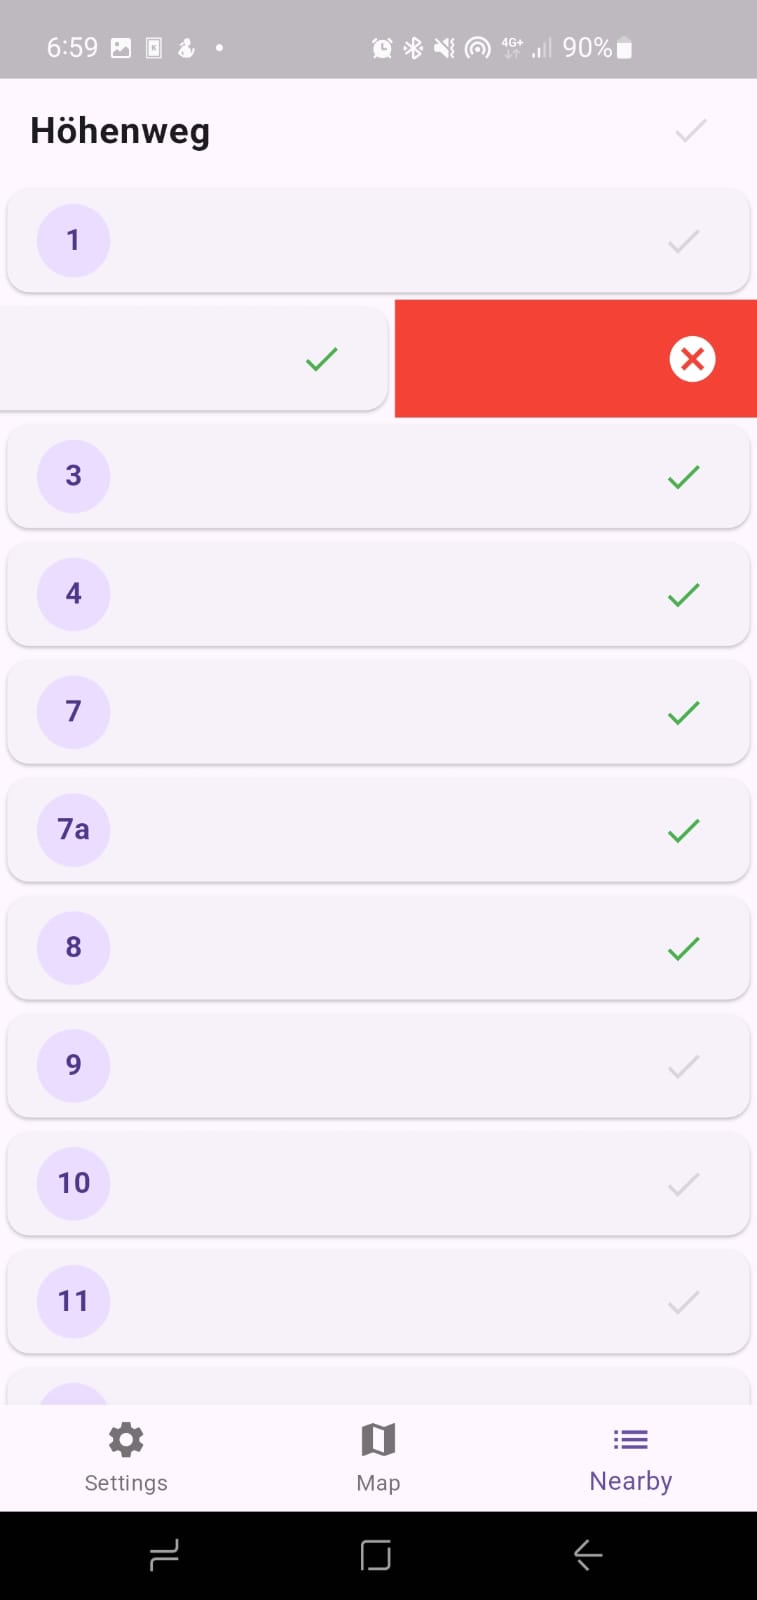
\includegraphics[width=\textwidth]{images/paul/listScreen/setIsVisitedFalse.jpeg}
      \caption{Same for setting it false}
  \end{minipage}
\end{figure}

\subsubsection{Future outlook for List Screen}
In the future, this component will likely be completely redesigned. This is due to the changed requirement that users want to be able to finer select the state of each address. This could be resolved by replacing the sliding gesture with a Dropbox. Then also a filter should be implemented so addresses that have a specific state, like \textit{visited, but nobody was home, will visit again}. Also, an \textit{onClick} event will be defined that opens the details' dialog.